\lez{1}{20-02-2020}{}
\subsubsection{Introduzione}%
Il corso è di astrofisica generale e darà una infarinatura generale degli argomenti principali dell'astrofisica.
\paragraph{Libro di testo}%
\texttt{Astrophysics for Physicists, Arnab Rai Choudhri}
\paragraph{Argomenti del corso}%
\begin{itemize}
	\item Trasporto radiativo.
	\item Stelle.
	\item Aggregati di stelle.
	\item Mezzo interstellare.
	\item Ammassi di galassie.
\end{itemize}
\subsection{Osservazione del cielo}%
\paragraph{Astrofisica}%
L'astrofisica è una scienza osservativa: non possiamo decidere di modificare il nostro "apparato", possiamo solo soltanto raccogliere informazioni attraverso le tecnologie di osservazione che abbiamo.\\
Le informazioni possono essere raccolte attraverso i diversi tipi di \textbf{messaggeri} che ci arrivano dal cosmo.\\
Il messaggero principale è la radiazione elettromagnetica, ultimamente si sono aggiunti altri portatori di informazioni: prima le particelle (neutrini) e successivamente le onde gravitazionali.\\ 
Resta il fatto che la stragrande maggioranza di informazioni che sappiamo dall'universo proviene dalla radiazione elettromagnetica.\\ 
Non potendo decidere quando i fenomeni avvengono sarà necessario sviluppare delle strategie che permettano di avere una sorta di \texttt{ridondanza osservativa} per riuscire ad accertare un supposto evento.

\paragraph{Osservazione della radiazione elettromagnetica}%
Fino all seconda guerra mondiale si osservava soltanto nella fascia dello spettro del visibile: tra i 4000 ed i 7000 \AA.\\
Successivamente, grazie all'invenzione del radar si sono aperte le regioni del Radio, X, Infrarosso, Gamma. Oggi si fanno osservazioni in tutto lo spettro. 

\paragraph{Lotta contro l'oscurità}%
La sfida è sempre stata nel vedere sorgenti deboli. Una sorgente può essere debole perchè è intrinsecamente debole (nana bianca antichissima, pianeti) oppure sorgenti intrinsecamente molto luminosi ma molto molto lontani. \\
Poter osservare oggetti sempre più lontani significa aumentare il numero di osservazione: posso avere più possibilità di osservare fenomeni mai visti prima e fare nuova fisica.\\
Per vedere oggetti sempre meno luminosi abbiamo bisogno di lenti dei telescopi sempre più grandi. Attualmente i telescopi ottici più grandi hanno diametri di 10 metri. L'ESA sta costruendo un telescopio di diametro di 39 metri. Avere un diametro più grande significa avere una sensibilità maggiore.

\subsection{Diffrazione e Seeing}%
\paragraph{Telescopi sempre più grandi}%
Aumentando la superficie della lente del telescopio aumenta la capacità di catturare luce e quindi la sensibilità del telescopio. Tuttavia questo non è l'unico motivo per cui si costruiscono telescopi sempre più grandi: c'è anche un motivo legato alla risoluzione del telescopio.\\
Quando guardiamo il cielo noi osserviamo degli angoli, le varie sorgenti che sono proiettate sulla volta celeste. La risoluzione è l'angolo più piccolo tra due sorgenti proiettate sulla volta celeste che mi permette di distinguerle.\\
Infatti per le dimensioni angolari degli oggetti luminosi nel cielo non sono trascurabili effetti di diffrazione. 
\paragraph{Diffrazione}%
Prendiamo il classico problema della fenditura:
\begin{figure}[H]
    \centering
    \incfig{diffrazione-da-una-fenditura}
    \caption{Diffrazione da una fenditura}
    \label{fig:diffrazione-da-una-fenditura}
\end{figure}
\noindent
Sappiamo che gli zeri della funzione di intensità $\frac{I}{I_0}$ sono nei punti:
\[
	\sin\theta = \frac{\lambda}{D}\cdot m \quad \quad m \text{ intero}
.\] 
Con il nostro telescopio abbiamo una situazione simile: abbiamo una stella lontana che irraggia. La sua luce entra in una fenditura circolare di diametro D data dal telescopio. Per il principio di Babinet sappiamo che anche in questo caso si crea una figura di interferenza che prenderà la seguente forma:
\begin{figure}[H]
	\centering
	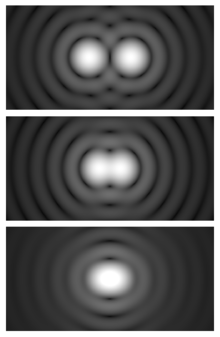
\includegraphics[width=0.2\textwidth]{figures/diffraction.png}
	\caption{\scriptsize Diffrazione al telescopio per due stelle al variare della risoluzione angolare.}
	\label{fig:diffraction}
\end{figure}
\noindent
Questa struttura di rifrazione ci permette di ridefinire il concetto di risoluzione, questa volta gli zeri sono in corrispondenza di alcuni numeri, il primo zero va ha $m=1.22$. \\
Il cerchio centrale, detto disco di Airy è importante perchè ci permette di discriminare due oggetti, questo risulta evidente in \hyperref[fig:diffraction]{Figura 2}\\
Prendendo angoli progressivamente più piccoli le figure di diffrazione tengono a sovrapporsi, il criterio per dire quando due sorgenti sono distinguibili è detto Criterio di Rayleigh: due sorgenti si dicono distinte quando hanno dischi di Hairy con centri che giacciono uno all'esterno dell'altro.
Quindi l'angolo minimo che riesco a risolvere sarà: 
\[
	\sin\theta_{min} \approx \theta_{min} =  1.22 \frac{\lambda}{D}
.\]
Quindi la risoluzione angolare di questo telescopio è data da questa formula. Per questo possiamo capire perchè è importante avere telescopi sempre più grandi.\\

Quando un telescopio arriva alla situazione in cui il limite di funzionamento è quello di diffrazione si dice che siamo nelle condizioni ottimali: quelle di Diffraction Limited (Hubble è in queste condizioni). 
\paragraph{Seeing}%
Sulla terra si può arrivare alla condizione ottimale del paragrafo precedente? In genere no per colpa della atmosfera, avente indice di diffrazione variabile è la maggiore fonte di disturbo.
\begin{figure}[H]
	\centering
	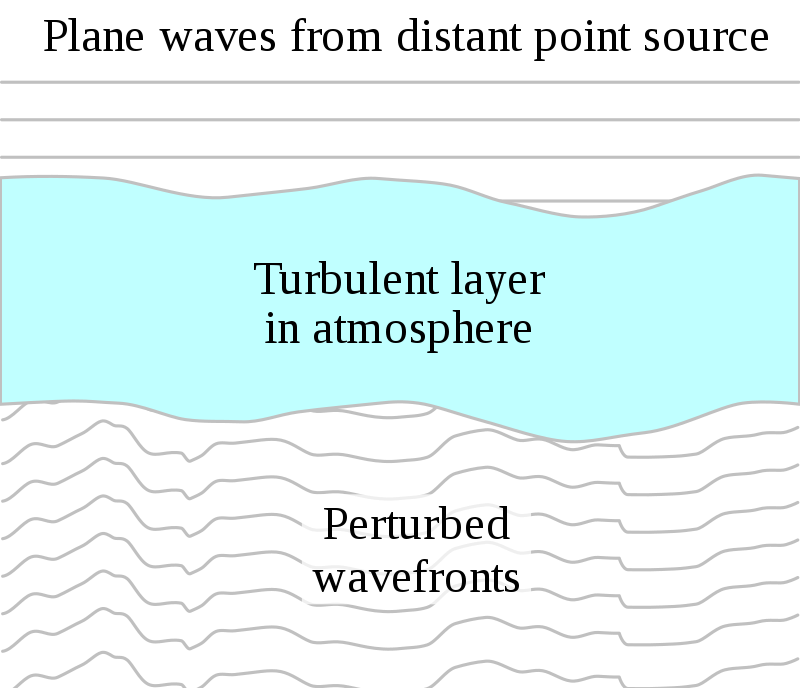
\includegraphics[width=0.3\textwidth]{figures/seeing.png}
	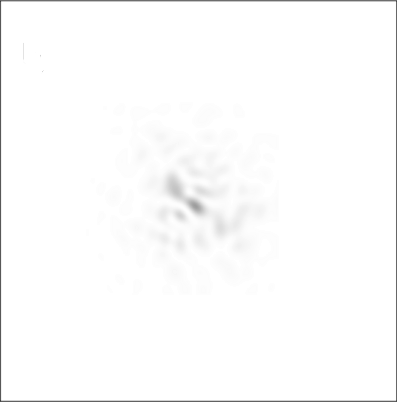
\includegraphics[width=0.2\textwidth]{figures/seeing-effect.png}
	\caption{\scriptsize A destra un possibile effetto sui fronti d'onda che attraversano l'atmosfera e a sinistra il risultato sulla stella agli occhi del telescopio, l'immagine risulta allargata e distorta.}
	\label{fig:figures-seeing-png}
\end{figure}
\noindent
Qual'è l'ordine di grandezza del Seeing? Se è buono si arriva al "secondo d'arco": $1''$. Nei siti migliori si arriva a $0.5''$.\\
Possiamo allora chiederci qual'è il valore del diametro del telescopio che mi produce un angolo di diffrazione minimo che corrisponde a quello del seeing. A quel punto non mi servirebbe a niente aumentare le dimensioni della lente: il seeing ci sarebbe comunque.\\
Nella luce visibile si ha $\lambda \approx 5000$ \AA, se prendiamo a questa lunghezza d'onda un angolo di $1''$ vediamo che il telescopio che raggiunge il limite del seeing è minuscolo: $D=$ 12 cm.\\
Perchè allora si costruiscono telescopi di 40 metri di diametro?
\begin{itemize}
	\item Per raccogliere comunque più luce.
	\item Per via dell'avvento della elettronica.
\end{itemize}
Esiste infatti un sistema detto ottica adattiva per correggere la presenza dell'atmosfera: si spara una sorgente laser in aria e si cercano di compensare elettronicamente l'effetto dell'atmosfera.
\paragraph{Lunghezza d'onda per cui oggi si ha la massima risoluzione angolare}%
Ha senso diminuire $\lambda$ fissando $D$, sembrerebbe quindi sensato andare nel Gamma, oggi invece si ha la risoluzione massima nel Radio grazie a Tecniche di interferometria: possiamo costruire array di telescopi che lavorano simultaneamente (si registra con orologi atomici l'arrivo del segnale): si arriva a  $D = 8600$ km (baseline molto lunga). Con questo metodo si arriva a risoluzioni di decine di micro arcosecondi! Questo è sicuramente il caso della foto del buco nero (30 arcosecondi). 
\begin{figure}[H]
	\centering
	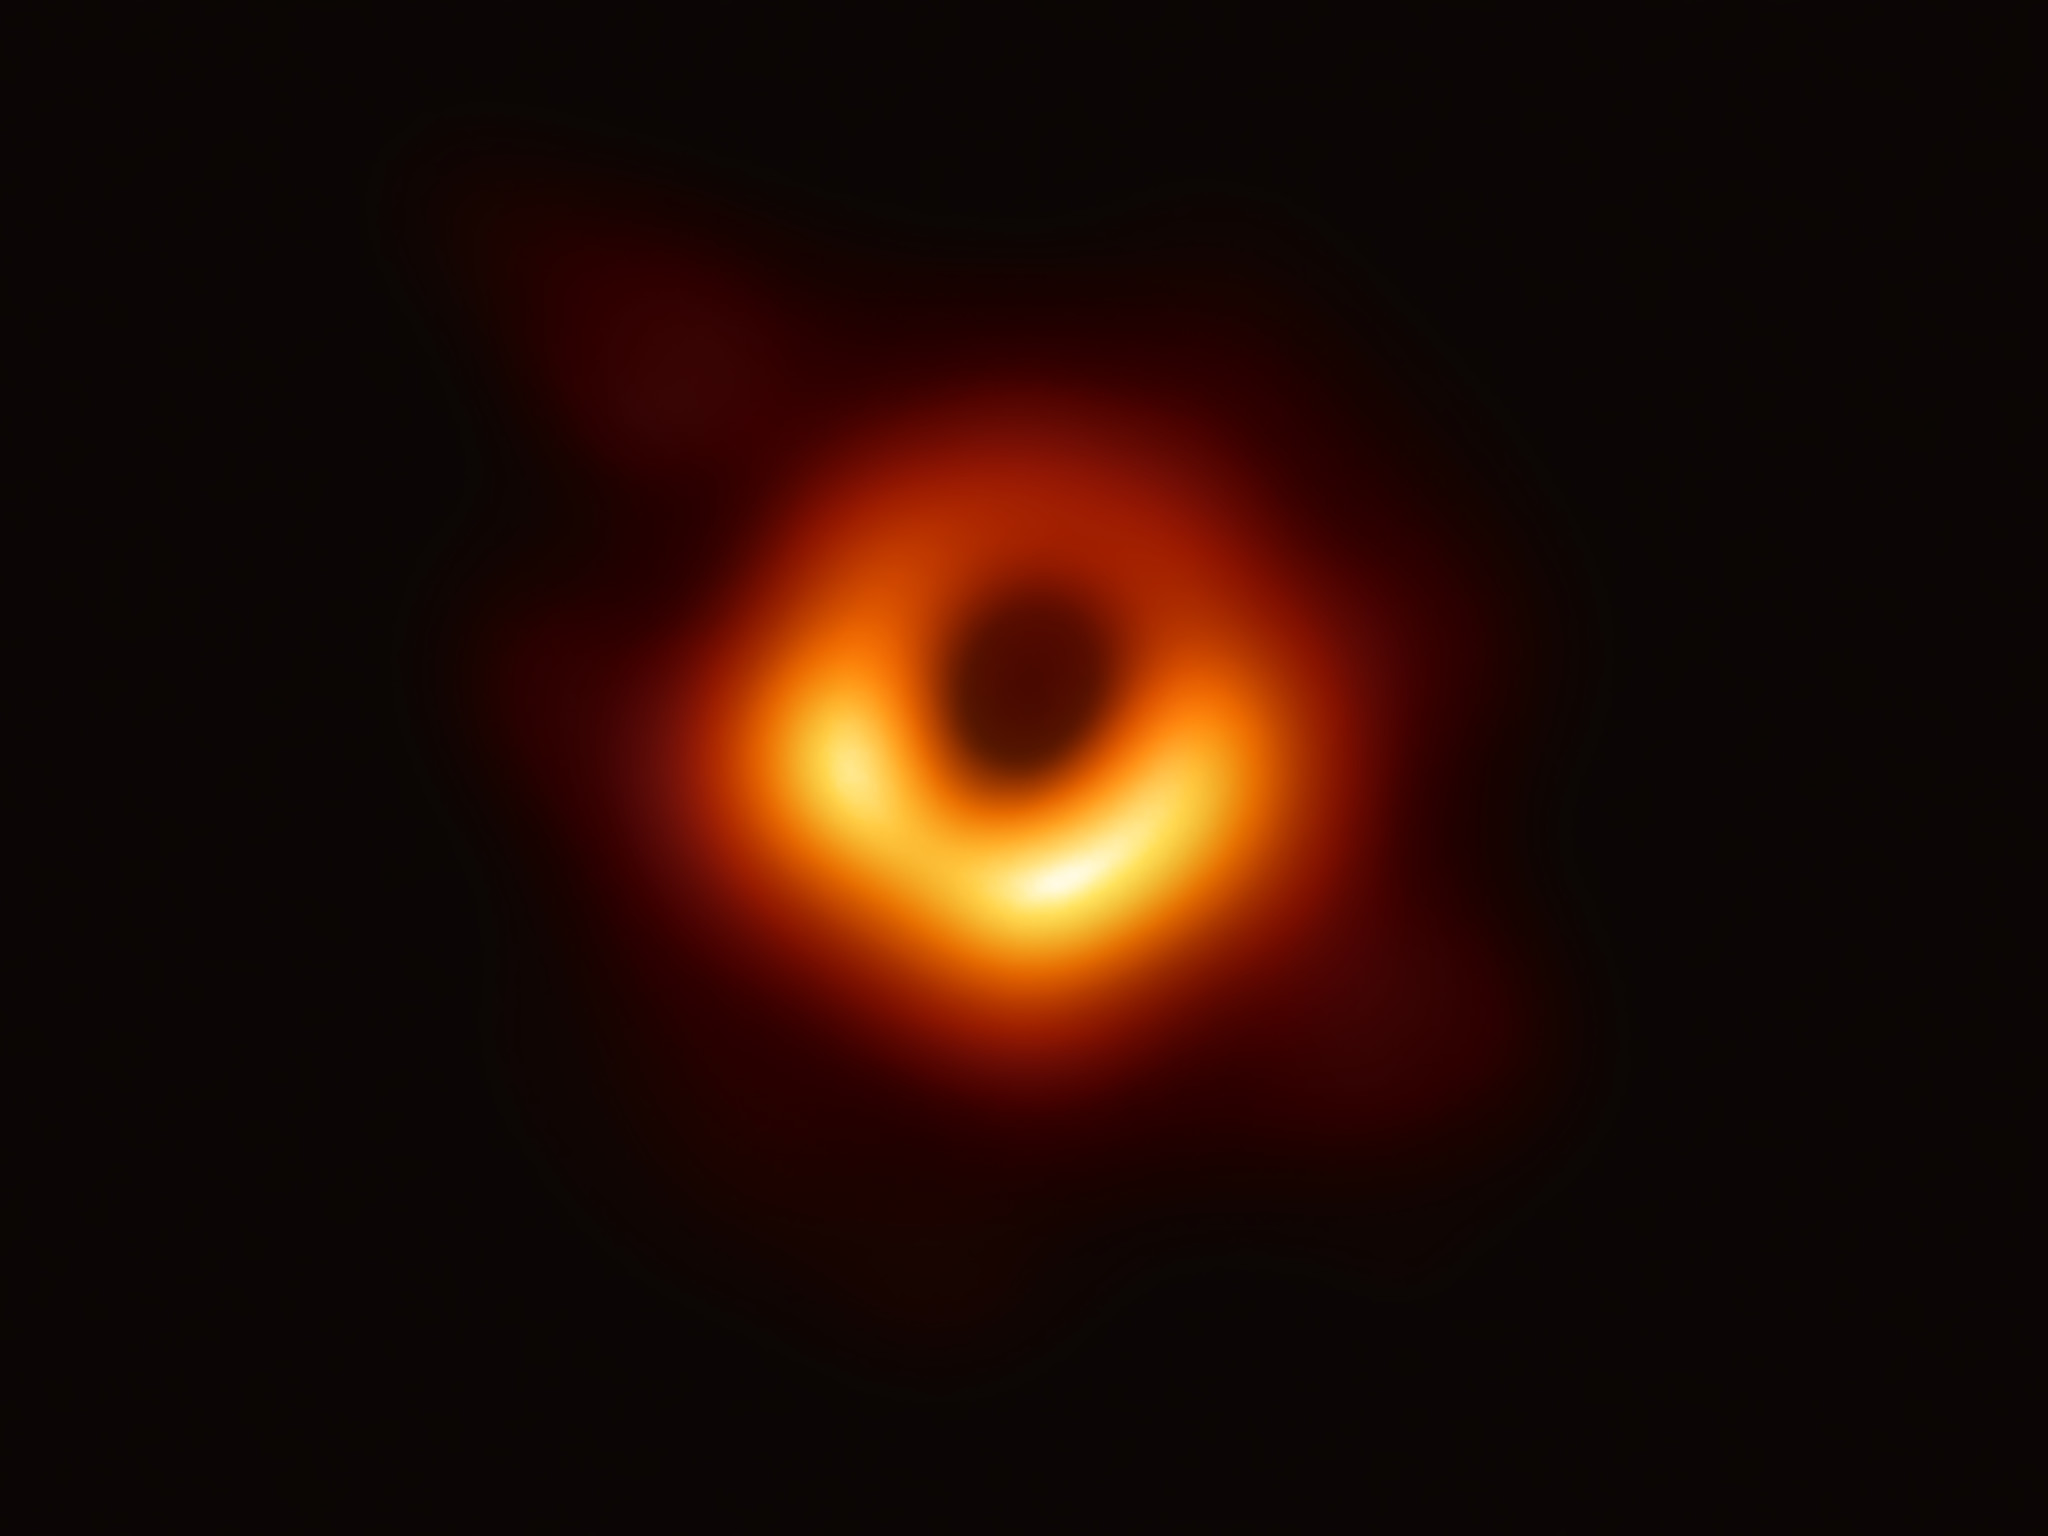
\includegraphics[width=0.4\textwidth]{figures/buconeroimmagine.jpg}
	\caption{Immagine del buco nero raccolta nel 2019}
	\label{fig:figures-buconeroimmagine-jpg}
\end{figure}

Ci sono alcune grandezze in astrofisica che non possono essere dimenticate ai fini di comprendere le grandezze di cui stiamo parlando. Queste grandezze alcune volte vengono anche adottate come unità di misura, visto che nella scala astrofisica le unità standard ridulterebbero decisamente incomprensibili!\\

\subsection{Massa del sole}%
Massa del sole: M\textsubscript{\(\odot\)} = $1.989 \cdot 10^{33}$ g $\approx 2 \cdot 10^{33} g$.\\
La massa minima per una stella è circa 0.08 M\textsubscript{\(\odot\)}\footnote{questa è la massa minima per innescare le reazioni termonucleari, chi non raggiunge queste dimensini (ma si avvicina) è detta Nana Bruna}, la massima si aggira attorno a 100 M\textsubscript{\(\odot\)}. \\
Le galassie hanno circa $10^{11}$ stelle, da cui per ottenere la massa di queste ultime si può mediare la massa a quella del sole con l'adeguato esponente. \\
Abbiamo anche aggregati di stelle (tipo Pleiadi, migliaglia di stelle) e più in là vedremo e studieremo gli ammassi di galassie.

\subsection{Distanze e metodo della parallasse}%
Raggio del sole: $R_{\odot} \approx 7 \cdot 10^{10} cm$.\\
La misura delle distanze in astronomia è complicata. Sono necessarie misure indirette spesso. Se voglio conoscere le dimensioni fisiche di un oggetto (trasformare angolo in distanza) ho bisogno di sapere quanto è distante! 
\paragraph{Metodo della parallasse}%
È l'unica misura diretta di distanza disponibile. È inoltre una misura di tipo geometrico:
\begin{figure}[H]
    \centering
    \incfig{metodo-della-parallasse}
    \caption{\scriptsize Metodo della parallasse: la stella risulta in diversi punti del cielo a seconda della posizione della terra.}
    \label{fig:metodo-della-parallasse}
\end{figure}
\noindent
Negli anni novanta abbiamo mandato un satellite che misurava fino ad un millesimo di secondo d'arco. La missione attuale più importante al riguardo è la GAIA: sta adesso mappando il cielo, quando tra qualche anno avrà finito si arriva a 30 microarcosecondi, purtoppo non si esce ancora dalla galassia con questo metodo.\\
Il metodo consiste in pratica nel vedere lo spostamento angolare dell'oggetto in momenti diversi dell'orbita di rotazione della terra attorno al sole: l'angolo di parallasse $\pi$ è la metà dell'angolo $\theta$
\[
	\frac{\theta}{2} = \pi
.\] 
Se conosciamo il raggio di orbita terrestre possiamo trovare la distanza della stella.\\
Noi conosciamo il raggio dell'orbita terreste medio \footnote{Grazie ad un trasponder radar montato sulla luna}, esso è l'unità astronomica A.U: $R \approx 1.5 \cdot 10^{13}$ cm.
\[
	\tan\left( \pi \right) \approx \pi  = \frac{R}{d}
.\] 

Il sistema solare (fino a nettuno) abbiamo una dimensione di 30 A.U. Fuori dal sistema solare è necessario definire un'altra unità di misura: il Parsec.\\
Un parsec è una distanza tale che la parallasse annua è 1'':
\[
	1 \text{ pc} \approx 3.09 \cdot 10^{18} \text{ cm} \sim 3.2 \text{ anni luce}
.\] 
La stella più vicina a noi ha una parallasse annua di 0.75'' l'anno (Proxima Centauri) che equivale a 1.3 pc. Misurare questi angoli è difficile in generale, gli angoli sono molto piccoli.\\
Le dimensioni di una galassia come la nostra invece sono:\\
\begin{figure}[H]
	\centering
	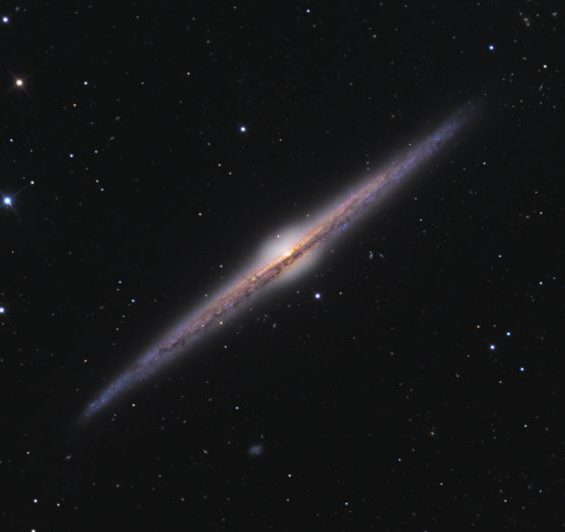
\includegraphics[width=0.4\textwidth]{figures/vialattea.jpeg}
	\caption{Rendering della via lattea vista dall'esterno.}
	\label{fig:figures-vialattea-jpeg}
\end{figure}
\[
	R_{disco} \sim 15 k\text{pc}
.\]
La distanza tra le galassie più vicine tra loro è dell'ordine del Mpc.\\
In genere le stelle invece distano tra loro di quantità dell'ordine dei parsec, è raro che collidano tra loro: l'una tra l'altra sono molto lontane rispetto alle dimensioni delle stelle stesse.\\ 
Non si può dire lo stesso per le galassie, ci sono solo pochi ordini di grandezza tra il raggio galattico è la distanza tra una galassia e l'altra, infatti le collisioni tra galassie sono più frequenti.\\
Le galassie più distanti sono dell'ordine del Gpc (questa è anche la scala delle dimensioni dell'universo).\\
\begin{figure}[H]
    \centering
    \incfig{scale-dell'universo}
    \caption{\scriptsize Scale dell'universo, il disegno è schematico e non è ovviamente in scala.}
    \label{fig:scale-dell'universo}
\end{figure}
\noindent

\subsection{Scale temporali dell'universo}%
Età del sole: $T_{\odot} = 4.57$ Gyr (Giga year). Questa è una delle poche datazioni misurata in modo diretto in astronomia, questa deriva dallo studio delle comete: queste sono rimaste intatte per miliardi di anni, queste vengono datate attraverso radiodatazioni.\\
Età dell'universo (dal Big Bang ad oggi): $T_{uni}= 13.8$ Gyr.

\subsection{Luminosità intrinseca, Candele campioni ed introduzione al trasporto radiativo}%
Negli anni '90 l'ESA ha mandato un satellite in grado di mappare decine di migliaglia di stelle attorno a noi distanti fino a 10 pc. GAIA è l'evoluzione di questo progetto, essa permettera di mappare tridimensionalmente la galassia. \\
Tuttavia anche con GAIA non si esce dalla galassia, quindi come si fa ad uscire? Come si misura la distanza se non sono in grado di misurare la parallasse?\\
Serve un metodo indiretto basato sul'concetto di \texttt{Candela campione}: un oggetto astronomico ci cui conosco la luminosità intrinseca.\\
Confrontando la luminosità intrinseca e la luminosità apparente osservata possiamo dedurre la distanza dell'oggetto. Questo è l'unico modo per misurare le distanze di oggetti all'esterno della via lattea. (Gli oggetti campione sono in genere le supernove).\\
Come faccio a partire dalla luminosità intrinseca a misurare la distanza?
\begin{figure}[H]
    \centering
    \incfig{propagazione-della-radiazione}
    \caption{Propagazione della radiazione}
    \label{fig:propagazione-della-radiazione}
\end{figure}
\noindent
Prendiamo una sorgente che irraggia come in \hyperref[fig:propagazione-della-radiazione]{Figura 8}. 
Se chiamiamo $F\left( r_1 \right) $ il flusso della radiazione che attraversa la superficie sferica concentrica alla sorgente di raggio $r_1$ allora:
\[
	F\left( r_1 \right) 4\pi r_1^2 = F\left( r_2 \right) 4\pi r_2^2 \implies F\left( r_2 \right) = F\left( r_1 \right) \left( \frac{r_1}{r_2} \right) ^2
.\] 
Abbiamo quindi una buona definizione di luminosità se ci mettiamo sul raggio $R$ della stella che irraggia:
\[
	F\left( R \right) 4\pi R^2  = L
.\] 
Tuttavia questa a livello pratico non è sufficiente. La radiazione non si propaga nel vuoto, è indispensabile quindi costruire una teoria del trasporto radiativo per tener di conto del mezzo interstellare. \\
Dobbiamo introdurre alcune grandezze per studiare il trasporto radiativo: \texttt{Intensità specifica monocromatica} (trattata dal punto di vista macroscopico \footnote{Valido quando la lunghezza d'onda che stiamo studiando sono piccole rispetto alle dimensioni del sistema, questo ci permette di immaginare che la radiazione si propaghi lungo dei raggi}):
\begin{figure}[H]
    \centering
    \incfig{figura-per-introdurre-lintensit-specifica}
    \caption{Figura per introdurre l'intensità specifica}
    \label{fig:figura-per-introdurre-lintensit-specifica}
\end{figure}
\noindent
Supponiamo di essere in un punto $\bs{r}$ all'istante $t$ e prendiamo in questo punto una superficie infinitesima elementare $dA$ orientata nella direzione $\hat{n}$ come in \hyperref[fig:figura-per-introdurre-lintensit-specifica]{Figura 9}. Ci interessa calcolare l'energia trasportata dalla radiazione elettromagnetica che attraversa la superficie $dA$ nella direzione $\hat{k}$ all'interno dell'angolo solido $d\Omega$ (inoltre deve essere monocromatica: tra $\nu$ e $d\nu$).\\
Quello che cerchiamo è dato da:
\[
	dE = I_{\nu}\left( \bs{r}, t,\bs{k} \right) \hat{k}\hat{n} dAdtd\Omega d\nu
	= I_{\nu}\left( \bs{r},t, \bs{k} \right) \cos\theta dA dt d\Omega d\nu
.\] 
Questa quantità è un flusso per unità di angolo solito: una brillanza superficiale. 
\[
	[I_{v}] = \text{[erg] cm $^{-2}$ s $^{-1}$ ster $^{-1}$ Hz $^{-1}$} 
.\] 
Dove ster è lo ster radiante.\\
$I_{\nu}$ è l'energia trasportata da un gruppo di fotoni che si muovono tutti nella stessa direzione contemporaneamente e tutti con la stessa frequenza.\\
È necessario notare che l'interazione tra radiazione e materia è anche argomento microscopico: il fotone interagisce anche con ioni, protoni, nuclei nel suo tragitto. Terremo conto con opportuni coefficienti il passaggio della radiazione nei vari mezzi quando scriveremo l'equazione del trasporto.\\
